\chapter{Defining refactoring-oriented clone types}\label{chap:clonetypes}
In section \ref{chap:backgroundclonetypes} we introduced the four clone types as defined in literature. These simple definitions are suitable for analysis of a codebase. Their detection results in simple to understand numbers to argue about a codebase. However, these clone types have a few flaws which makes it hard to argue to what extend two fragments of code can and should be refactored. For each of type 1-3 clones~\cite{roy2007survey} we list our solutions to their shortcomings to increase the chance that we can refactor the clone while improving the design.

We also look into clone detection tools for their suitability to support the proposed clone type definitions. We selected a few criteria  Most clone detection tools support these definitions of clone types. However, many of these tools use a vastly different approach. A study by Saini et al \cite{saini2018towards} outlines different clone detection tools and compares their results for each of type 1-3 clones. Even though they operate on the same type definitions, the tools used in this study yield different results.

\section{Shortcomings of clone types}
Clone types 1-3 (further explained in section \ref{chap:backgroundclonetypes}) allow reasoning about the duplication in a software system. Clones by these definitions can relatively easily and efficiently be detected. This has allowed for large scale analyses of duplication~\cite{livieri2007very}. However, these clone type definitions have shortcomings which makes the clones detected in correspondence with these definitions less valuable for (automated) refactoring purposes.

In this section, we discuss the shortcomings of the different clone type definitions. Because of these shortcomings, clones found by these definitions are often found to require additional judgment whether they should and can be refactored.

\subsection{Type 1 clones}\label{sec:type1}
Type 1 clones are \textit{identical clone fragments except for variations in whitespace and comments} \cite{roy2007survey}. This allows for the detection of clones that are the result of copying and pasting existing code, along with other reasons why duplicates might get into a codebase.

Type 1 clones are implemented as textual equality between code fragments (except for whitespace and comments) by most clone detection tools~\cite{kamiya2002ccfinder, semura2017ccfindersw, roy2008nicad, svajlenko2016bigcloneeval, svajlenko2014evaluating}. Although textually equal, method calls can still refer to different methods, type declarations can still refer to different types and variables can be of a different type. In such cases, refactoring opportunities could be invalidated. This can make type 1 clones less suitable for refactoring purposes, as they require additional judgment regarding the refactorability of such a clone. When aiming to automatically refactor clones, applying refactorings to type 1 clones is bound to be error prone and can result in an uncompilable project or a difference in functionality.

\begin{figure}[H]
\begin{parcolumns}{2}
\colchunk[1]{
\begin{javacode}
package com.sb.game;

import java.util.List;

public class GameScene
{
|\highlightYellow|	public void addToList(List l) {
|\highlightYellow|		l.add(getClass().getName());
|\highlightYellow|	}

	public void addTen(int x) {
|\highlightYellow|		x = x + 10;
|\highlightYellow|		Notifier.notifyChanged(x);
|\highlightYellow|		return x;
	}
}
\end{javacode}}
\colchunk[2]{
\begin{javacode}
package com.sb.fruitgame;

import java.awt.List;

public class LoseScene
{
|\highlightYellow|	public void addToList(List l) {
|\highlightYellow|		l.add(getClass().getName());
|\highlightYellow|	}

	public void concatTen(String x) {
|\highlightYellow|		x = x + 10;
|\highlightYellow|		Notifier.notifyChanged(x);
|\highlightYellow|		return x;
	}
}
\end{javacode}}
\end{parcolumns}
\caption{Example of a type 1 clone that is functionally different.}
\label{fig:type1}
\end{figure}

In the example in figure \ref{fig:type1}, we see a type 1 clone displaying two clone classes. Defining an automatic way to refactor these clone classes is nearly impossible, as both cloned fragments describe different functional concepts. The first cloned fragment is a method that adds something to a \texttt{List}. However, the \texttt{List} objects to which something is added are different. Looking at the \texttt{import} statement above the class, one fragment uses the \texttt{java.util.List} and the other uses the \texttt{java.awt.List}. Both happen to have an \texttt{add} method, but apart from that their implementation is completely different.

The second cloned fragment shows how equally named variables can have different types and thus yield different functional concepts. The cloned fragment on the left adds a specific amount to an integer. The cloned fragement on the right concatenates a number to a String.

This shows that not all type 1 clones can easily be automatically refactored. In section \label{chap:type1rclones} we describe an alternate approach towards detecting type 1 clones, which results in only clones that can be refactored.

\subsection{Type 2 clones}\label{sec:type2}
Type 2 clones are \textit{structurally/syntactically identical fragments except for variations in identifiers, literals, types, layout and comments}~\cite{roy2007survey}. This definition allows for the reasoning about code fragments that were copied and pasted, and then slightly modified. However, the definition does not adequately differentiate between slight modification and completely different fragments that just happen to have the same structure.

For refactoring purposes, this definition is unsuitable; if we allow any change in identifiers, literals, and types, we cannot distinguish between different variables, different types and different method calls anymore. This could render two methods that have an entirely different functionality as clones. Merging such clones can be harmful instead of helpful.

\begin{figure}[H]
\begin{parcolumns}{2}
\colchunk[1]{
\begin{javacode}
|\highlightYellow|public boolean redCircles
|\highlightYellow|          (List<Circle> circles){
|\highlightYellow|	return circles.stream()
|\highlightYellow|           .allMatch(Shape::isRed);
|\highlightYellow|}
\end{javacode}}
\colchunk[2]{
\begin{javacode}
|\highlightYellow|public Apple getEdibleApple
|\highlightYellow|         (Basket<Apple> basket){
|\highlightYellow|	return basket.getFruit()
|\highlightYellow|        .getApple(Fruit::notEaten);
|\highlightYellow|}
\end{javacode}}
\end{parcolumns}
\caption{Example of a type 2 clone with high variability between fragments.}
\label{fig:type2}
\end{figure}

The example in figure \ref{fig:type2} shows a type 2 clone class. Both methods are, except for their matching structure, completely different in functionality. They operate on different types, call different methods, return different things, etc. Having such a method flagged as a clone does not provide much useful information.

When looking at refactoring, type 2 clones can be difficult to refactor. For instance, if we have variability in types, the code can describe operations on two completely dissimilar types. Type 2 clones do not differentiate between primitives and reference types, which further undermines the usefulness of clones detected by this definition.

\subsection{Type 3 clones}\label{sec:type3}
Type 3 clones are \textit{copied fragments with further modification (with added, removed or changed statements)}~\cite{roy2007survey}. Detection of clones by this definition can be hard, as it may be hard to detect whether a fragment was copied in the first place if it was severely changed. Because of this, most clone detection implementations of type 3 clones work on the basis of a similarity threshold~\cite{roy2008nicad,ragkhitwetsagul2019siamese,jiang2007deckard,semura2017ccfindersw}. This similarity threshold has been implemented in different ways: textual similarity (for instance using Levenshtein distance)~\cite{lavoie2011automated}, token-level similarity~\cite{sajnani2016sourcerercc} or statement-level similarity~\cite{kamalpriya2017enhancing}.

Having a definition that allows for any change in code poses serious challenges on refactoring. A Levenshtein distance of one can already change the meaning of a code fragment significantly, for instance, if the name of a type differs by a character (and thus referring to different types).

\section{Refactoring-oriented clone types}\label{sec:rtypes}
To resolve the shortcomings of clone types as outlined in the previous section, we propose alternative definitions for clone types directed at detecting clones that can and should be refactored. We have named these clones T1R (type 1R), T2R and T3R clones. These definitions address problems of the corresponding literature definitions. The ``R'' stands for refactoring-oriented (and may be less useful for other analyses).

\subsection{Type 1R clones} \label{sec:type1r}
To solve the issues identified in section \ref{sec:type1}, we introduce an alternative definition: cloned fragments have to be both textually \textit{and} functionally equal. Like type 1 clones, type 1R clones do not consider comments and whitespace. Therefore, T1R clones are a subset of type 1 clones.

We check functional equality of two fragments by validating the equality of the fully qualified identifier (FQI) for referenced types, methods and variables. If an identifier is fully qualified, it means we specify the full location of its declaration (e.g. \texttt{com.sb.fruit.Apple} for an \texttt{Apple} object).

\subsubsection{Referenced Types}
Many object-oriented programming languages (like Java, Python and C\#) require the programmer to import a type (or the class in which it is declared) before it can be used. Based on what is imported, the meaning of the name of a type can differ. For instance, if we import \texttt{java.util.List}, we get the interface which is implemented by all list datastructures in Java. However, importing \texttt{java.awt.List}, we get a listbox GUI component for the Java Abstract Window Toolkit (AWT). To be sure we compare between equal types, type 1R clones compare the FQI for all referenced types.

\subsubsection{Called methods}
A codebase can have several methods with the same name. The implementation of these methods might differ. When we call two methods with an identical name, we can in fact call different methods. This is another reason that textually identical code fragments can differ functionally.

Because of this, for type 1R clones, we compare the fully qualified method signature for all method references. A fully qualified method signature consists of the fully qualified name of the method, the fully qualified type of the method plus the fully qualified type of each of its arguments. For instance, an \texttt{eat} method could become \texttt{com.sb.AppleCore com.sb.fruitgame.Apple.eat(com.sb.fruitgame.Tool)}.

\subsubsection{Variables}
In typed programming languages, each variable declaration should declare a name and a type. When we reference a variable, we only use its name. If, in different code fragments, we use variables with the same name but different types, the code can be functionally unequal but still textually equal. As an example, see the code in figure \ref{fig:type2variables}.

\begin{figure}[H]
\begin{parcolumns}{2}
\colchunk[1]{
\begin{javacode}
public int addFive(int x){
|\highlightYellow|	return x + 5;
}
\end{javacode}}
\colchunk[2]{
\begin{javacode}
public String appendFive(String x){
|\highlightYellow|	return x + 5;
}
\end{javacode}}
\end{parcolumns}
\caption{Variables with different types but the same name.}
\label{fig:type2variables}
\end{figure}

The body of both methods in figure \ref{fig:type2variables} is equal. However, their functionality is not. The first method adds two numbers together and the other concatenates an integer to a String.

For type 1R clones variable references should be compared by both type and name.

\subsection{Type 2R clones} \label{sec:type2r}
Type 2R clones are modelled after type 2 clones, which allow any change in identifiers, literals, types, layout, and comments. For refactoring purposes, this definition is unsuitable; if we allow any change in identifiers, literals, and types, we cannot distinguish between different variables, different types and different method calls anymore. This could render two methods that have an entirely different functionality as clones (as shown in figure \ref{fig:type2} previously).

We tackle these problems with type 2R clones to be able to detect such clones that can and should be refactored. Type 1R clones are a subset of type 2R clones, meaning that each node found as cloned for type 1R will also be found as cloned for type 2R. Similar to type 1R, for type 2R we consider the fully qualified identifiers of type-, method- and variable-references. Additionally, type 2R clones allow variability in a controlled set of expressions and identifiers. The identifiers and expressions in which we allow variability must have one of the following properties:
\begin{itemize}
  \item We allow a difference in identifiers between cloned fragments if it has no impact on the refactoring process.
  \item We allow a difference in expressions between cloned fragments if the expression can be extracted to a method argument when applying the ``Extract Method'' refactoring.
\end{itemize}

Allowing variability between expressions includes a tradeoff. When many expressions vary between cloned the refactored method might require many additional arguments. Because of that, we constrain this variability by a threshold, which is explained in more detail in section \ref{sec:variabilitythreshold}.%to limit the negative effect on system design of variability in these expressions after refactoring.

\subsubsection{Allow any variability in some identifiers}
When refactored, some identifiers have no detrimental effect on the design if they vary between cloned instances. This section explains several patterns of variability that we can allow between cloned fragements without changing the method by which the fragments can be refactored.

\paragraph{Declaration names}
The names of declarations describe the implementation of their body. Examples of declarations are:
\begin{itemize}
  \item Class declaration
  \item Method declaration
  \item Interface declaration (not all languages have a separate declaration for these)
  \item Enumeration declaration (not all languages have a separate declaration for these)
  \item Annotation declaration (not all languages support these)
  \item Etc.
\end{itemize}
If two declaration bodies and signatures are cloned, but their names differ, one of both names should be redundant. When refactoring such clones, we can choose one instance to keep and one to remove. Such a refactoring doesn't affect maintainability in any other way than refactoring a type 1R clone would. Because of this, type 2R allows any variability in declaration names. However, this will only open up a good refactoring opportunity if the entire body and signature of these declarations are cloned.

\paragraph{Variable names}
Cloned code fragments using variables with different names can be refactored without a design tradeoff if the following conditions apply:

\begin{itemize}
  \item The cloned variables are locally defined or the refactoring method used requires extraction to method argument anyways.
  \item The cloned variables have the same type.
  \item The cloned variables are used at the same places in cloned fragments.
\end{itemize}

\todo{Show examples}

\subsubsection{A threshold for variability in literals, variables and method calls}\label{sec:variabilitythreshold}
Type 2 clones allow any variability in literals, variables and method identifiers. However, this information tells a lot about the meaning of the code fragment. Most clone detection tools do not differentiate between a type 2 clone that differs by a single literal/identifier and one that differs by many \cite{roy2009comparison}. However, this does have a big impact on the meaning of the code fragment.

For type 2R clones we define a threshold for variability in literals, variables and method calls. We calculate the variability in literals, variables and method calls using the following formula:

\begin{equation}\label{eq:type2r}
\text{T2R Variability}=\frac{\text{Number of different expressions}}{\text{Total number of expressions in clone instance}}*100
\end{equation}

In this formula, \textit{number of different expressions} refers to the number of literals, variables and method calls that differ from other clone instances in a clone class. We divide this by the total number of expressions in the clone instance. Based on this threshold, we decide whether a clone should be considered for refactoring. A concrete example of applying this formula to calculate a threshold is given in \ref{sec:t2rcheckglobalthres}.

\paragraph{Literal and variable variability}\label{sec:t2rliteralandvariable}
We allow only variability in the value of literals and variables, but not in their types. This is because a difference in literal/variable type may have a big impact on the refactorability of the cloned fragment. When we refactor different literals/variables that have both the same type, in case of an ``Extract Method'' refactoring, we have to create a parameter for this literal and pass the corresponding literal/variable from cloned locations. However, if two literals have different types, this might not be possible (or will have a negative effect on the design of the system). This is because a lot of variability in literals will result in more parameters required in the extracted method, which is detrimental for the design of the system.

Consider the example in figure \ref{fig:type2literal}. In this example, the two methods have two literals that differ between them. We can perform an ``Extract method'' refactoring on these to get the result that is displayed on the right. In this process, we create a method parameter for the corresponding literal.

\begin{figure}[H]
\begin{parcolumns}{2}
\colchunk[1]{
\begin{javacode}
// Original
void doABC(){
	doA();
	doB("abc");
	doC();
}

void doDEF(){
  doA();
  doB("def");
  doC();
}
\end{javacode}}
\colchunk[2]{
\begin{javacode}
// Refactored
void doABC(){
	doThis("abc");
}

void doDEF(){
	doThis(s, "def");
}

void doThis(String letters){
  doA();
  doB(letters);
  doC();
}
\end{javacode}}
\end{parcolumns}
\caption{Literal variability refactored.}
\label{fig:type2literal}
\end{figure}

\paragraph{Method call variability}
Most modern programming languages (like Java, Python and C\#) allow to pass method references as a parameter to a method. This helps reducing duplication, as it is possible to refactor two code fragments which differ only by a method call. However, a method call does often not consist of a single token (like variables and literals). For instance, a method call \texttt{System.out.println()} consists of several segments: a type reference to the \texttt{System} type, a reference to the static \texttt{out} field and a call of the \texttt{println()} method.

Type 2R clones allow called methods to vary as long as they have the same argument types and return type. As with type 1R clones, these types are compared using their fully qualified identifiers. An example of this is shown in figure \ref{fig:type2method}. In this example, we have two methods (\texttt{System.out.println} and \texttt{myFancyPrint}). We use the ``Extract Method'' refactoring method to extract a new method and use a parameter to pass the used method.

The method call variability property of type 2R clones imply that type 2R clones are not a subset of type 2 clones. Because methods calls can have a different structure, type 2R clones can be structurally slightly different. The example as shown in figure \ref{fig:type2method} can be a type 2R clone (dependent on the thresholds used), but is not a type 2 clone.

\begin{figure}[H]
\begin{parcolumns}{2}
\colchunk[1]{
\begin{javacode}
// Original
void doABC(){
	doA();
	doB();
	doC();
}

void doADC(){
  doA();
  doD();
  doC();
}
\end{javacode}}
\colchunk[2]{
\begin{javacode}
// Refactored
void doABC(){
	doThis(this::doB);
}

void doADC(){
	doThis(this::doD);
}

void doThis(Runnable r){
  doA();
  r.run();
  doC();
}
\end{javacode}}
\end{parcolumns}
\caption{Method variability refactored.}
\label{fig:type2method}
\end{figure}

\subsection{Type 3R clones}\label{sec:type3r}
Type 3 clones allow any change in statements, often bounded by a similarity threshold. This means that type 3 clones allow the inclusion of a statement that is not detected by type 1 or 2 clone detection. When looking at how we can refactor a statement that is not included by one clone instance but is in another, we find that we require a conditional block to make up for the difference in statements. See figure \ref{fig:type3} for an example of such a clone.

\begin{figure}[H]
\begin{parcolumns}{2}
\colchunk[1]{
\begin{javacode}
// Original
void doCwithA(){
	int a = getA();
	doC(a);
}

void multiplyA(){
  int a = getA();
  a *= 5;
  doC(a);
}
\end{javacode}}
\colchunk[2]{
\begin{javacode}
// Refactored
void doCwithA(){
	modifyA(false);
}

void multiplyA(){
	modifyA(true);
}

void modifyA(boolean multiply){
  int a = getA();
  if(multiply) a *= 5;
  doC(a);
}
\end{javacode}}
\end{parcolumns}
\caption{Added statement between cloned fragments refactored.}
\label{fig:type3}
\end{figure}

In figure \ref{fig:type3} a single statement is added. This statement is found in between cloned lines. There is a \textit{gap} of non-cloned lines in between two clone classes. The following rules apply to this gap:

\begin{itemize}
  \item \textbf{The difference in statements must bridge a gap between two clones that were valid by the original thresholds}. This entails that, different from type 3 clones, the difference in statements cannot be at the beginning or the end of a cloned block. It is rather somewhere within, as it must bridge two existent clones.
  \item \textbf{The size of the gap between two clones is limited by a threshold.} This threshold is calculated by taking the percentage of the number of statements in the gap over the number of statements that both clones that are being bridged span.
  \item \textbf{The gap may not span a partial block.} To make sure that the T3R clone can be refactored, we do not allow the gap to span a part of a block, for instance, the declaration and a part of the body of a for-loop. The reason for this is that it is not possible to wrap a partially spanned block in a single conditional statement. We could, however, use multiple conditional blocks (one for each block spanned), but due to the detrimental effect on the design of the code (as each conditional block adds a certain complexity), we decided not to allow this for T3R clones.
\end{itemize}

\subsubsection{Gap Threshold}
\begin{equation}\label{eq:type3r}
\text{T3R Gap Size}=\frac{\text{Number of nodes in gap}}{\text{Number of nodes in clones}}*100
\end{equation}

When applying this formula with the example given in figure \ref{fig:gappedclones}, we get a gap size of 25\%:

\begin{equation}\label{eq:type3r}
\text{T3R Gap Size}=\frac{\text{|\{doC()\}|}}{\text{|\{doA(), doB(), doD(), doE()\}|}}*100 = \frac{\text{1}}{\text{4}}*100 = 25\%
\end{equation}

\begin{figure}[H]
\begin{parcolumns}{2}
\colchunk[1]{
\begin{javacode}
public void doStuff(){
|\highlightYellow|  doA(); // Clone instance of
|\highlightYellow|  doB(); // two statements
  doC(); // Gap of one statement
|\highlightBlue|  doD(); // Clone instance of
|\highlightBlue|  doE(); // two statements
}
\end{javacode}}
\colchunk[2]{
\begin{javacode}
public void doStuff(){
|\highlightYellow|  doA(); // Clone instance of
|\highlightYellow|  doB(); // two statements
  doF(); // Gap of one statement
|\highlightBlue|  doD(); // Clone instance of
|\highlightBlue|  doE(); // two statements
}
\end{javacode}}
\end{parcolumns}
\caption{Gapped clones.}
\label{fig:gappedclones}
\end{figure}

Apart from this threshold, the gap in between clones may not span over different blocks. Look at figure \ref{fig:type3invalid} for an example of this. We cannot refactor both statements into a single conditional block. We could however use two conditional blocks, but due to the detrimental effect on the design of the code (as each conditional block adds a certain complexity), we decided not to allow this for type 3R clones.

\begin{figure}[H]
  \centering
  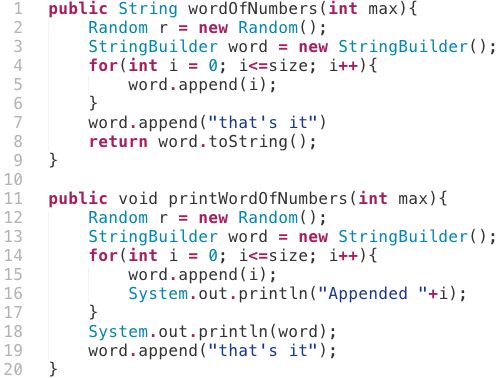
\includegraphics[width=0.6\columnwidth]{img/type3invalid}
  \caption{Statements between clones in different blocks.}
  \label{fig:type3invalid}
\end{figure}

\subsection{Clone types summarized}
The given clone definitions (types 1R, 2R and 3R) are refactoring-oriented in the sense that they were designed after the literature type definitions but with a concrete refactoring opportunity in mind. Summarized, these types can be explained as follows:

\begin{itemize}
\item \textbf{Type 1R:} Allows no difference between cloned fragments (both functionally and textually), making it possible to refactor both fragments to a method call that contains the code of both locations. \\
\item \textbf{Type 2R:} Allows difference between cloned fragments in a controlled set of expressions. Refactoring opportunities for these controlled features are known, allowing refactoring with a minor tradeoff. \\
\item \textbf{Type 3R:} Allows any difference. When refactored, this difference must be wrapped in a conditionally executed block, which entails a major tradeoff.
\end{itemize}

Regarding the nodes found as cloned by these clone type definitions, there exists a subset relation between all types:

\begin{equation}\label{eq:typerelation}
\text{Cloned nodes} = T1R \subseteq T2R \subseteq T3R
\end{equation}

Comparing these clone type definitions to the ones used in literature, type 1R clones are a subset of type 1 clones. However, this subset relation does not exist for type 2R and 3R clones. This is because these definitions allow variability in multi-token method calls, which type 2 and type 3 do not allow. Because of that, the following is true for these clone types:

\begin{equation}\label{eq:typerelation2}
\text{Cloned nodes} = T1R \subseteq T1 \text{, but } T2R	\nsubseteq T2 \text{ and } T3R \nsubseteq T3
\end{equation}

\subsection{The challenge of detecting these clones}\label{chap:challenge}
To detect each type of clone, we need to parse the fully qualified identifier of all types, method calls and variables. This comes with serious challenges, regarding both performance and implementation. Also, to be able to parse all fully qualified identifiers, and trace the declarations of variables, we might need to follow cross file references. The referenced types/variables/methods might even not be part of the project, but rather of an external library or the standard libraries of the programming language. All these factors need to be considered for the referenced entity to be found, on the basis of which a fully qualified identifier can be created.

\section{Suitability of existing Clone Detection Tools for detecting these clones}
\todo{Is this still up to date?}
\label{ch:tool-overview}
We conducted a short survey on (recent) clone detection tools that we could use to analyze refactoring possibilities. The results of our survey are displayed in table~\ref{table:dettools}. We chose a set of tools that are open source and can analyze a popular object-oriented programming language. Next, we formulate the following four criteria by which we analyze these tools:
\begin{enumerate}
    \item \textbf{Should find clones in any context.} Some tools only find clones in specific contexts, such as only method level clones. We want to perform an analysis of all clones in projects to get a complete overview.
\item \textbf{Finds clone classes in control projects.} We assembled a number of control projects to assess the validity of clone detection tools.
\item \textbf{Can analyze resolved symbols.} When detecting the types proposed in section~\ref{sec:rtypes}, it is important that we can analyze resolved symbols (for instance a type reference). The rationale for this is further explained in~\ref{chap:challenge}.
\item \textbf{Extensive detection configuration.} Detecting our clone definitions, as proposed in section~\ref{sec:rtypes}, require to have some understanding about the meaning of tokens in the source code (whether a certain token is a type, variable, etc.). The tool should recognize such structures, in order for us to configure our clone type definitions in the tool.
\end{enumerate}

\begin{table}[H]
 \begin{center}
  \caption{Our survey on clone detection tools.} \label{table:dettools}
  \medskip
\begin{tabular}{|l|l|l|l|l|l|}
\hline
\textbf{Clone Detection Tool} & \textbf{(1)} & \textbf{(2)} & \textbf{(3)} & \textbf{(4)} \\ \hline
Siamese~\cite{ragkhitwetsagul2019siamese} &  &             &             & \checkmark            \\ \hline
NiCAD~\cite{roy2008nicad, cordy2011nicad} & \checkmark                             & \checkmark            &             &             \\ \hline
CPD~\cite{roy2009comparison} & \checkmark & \checkmark            &             &             \\ \hline
\begin{tabular}[c]{@{}l@{}}CCFinder~\cite{kamiya2002ccfinder}\\ D-CCFinder~\cite{livieri2007very}\end{tabular} & \checkmark  & \checkmark   &    &   \\ \hline
CCFinderSW~\cite{semura2017ccfindersw}   & \checkmark     &             &             & \checkmark            \\ \hline
\begin{tabular}[c]{@{}l@{}}SourcererCC~\cite{sajnani2016sourcerercc}\\ Oreo~\cite{saini2018oreo}\end{tabular} & \checkmark    &             &             & \checkmark            \\ \hline
BigCloneEval~\cite{svajlenko2016bigcloneeval}  & \checkmark  & \checkmark   &             &             \\ \hline
Deckard~\cite{jiang2007deckard} & \checkmark   &             & \checkmark            &             \\ \hline
Scorpio~\cite{higo2013revisiting, kamalpriya2017enhancing} & \checkmark   &     & \checkmark  & \checkmark   \\ \hline
\end{tabular}
\end{center}
\end{table}

None of the state-of-the-art tools we identified implement all our criteria, so we decided to implement our own clone detection tool, which is further described in the next chapter.
